For starting, remark that although a matrix $t\in\HOM{\LREL_!}{X}{Y}$ yields a linear map $\Lawv^{!X}\to\Lawv^Y$, by exploiting the coKleisli structure we can also ``express it in the base $X$'', i.e.\ see it as a \emph{non-linear} map $t^!:\Lawv^X\to\Lawv^Y$, by setting $t^!(x):=t\circ_! x$. %(we are identifying $\Lawv^X$ with the set $\HOM{\LREL_!}{\emptyset}{X}$ of the \emph{points} of $X$).
Concretely, we have $t^!(x)_b=\inf_{\mu\in !X} \set{\mu x+ t_{\mu,b}}$, where $\mu x:=\sum_{a\in X} \mu(a)x_a$.
In this section we establish some topological and metric properties of such functions, this way highlighting the rich and interesting topological and metric structure of the category $\LREL_{!}$.
As we explain in a moment, those are generalised \emph{tropical Laurent series} (\emph{tLs} for short), and as the literature in tropical mathematics is often recent (e.g.~\cite{Porzio2021}), several results we prove in this section are, to our knowledge, new.

%
%In this section we study the tropical Laurent series $\Lawv^X\to \Lawv ^Y$ from the viewpoint of analysis.

\subsection{From tropical polynomials to tLs}\label{sec:4A}

A \emph{tropical polynomial} is a piece-wise linear function $f:\Lawv\to \Lawv$ of the form $f(x)=\min_{0\leq j\leq n}\{i_{j}x+c_{i_{j}}\}$, where $i_{j}\in\N$ and $c_{i_{j}}\in\Lawv$.
For example, the polynomials $\varphi_{n}(x)=\min_{0\leq j\leq n}\{jx+2^{-j}\}$
are illustrated in Fig.~\ref{fig:plot1} for $0\leq n \leq 4$.
A \emph{tropical root} of a tropical polynomials $\varphi$ is a point $x\in \Lawv$ where $\varphi$ is not differentiable. In other words, the roots of $\varphi$ are the points where the minimum defining $\varphi$ is attained at least twice (i.e.~where the slope of $\varphi$ changes).
For instance, the tropical roots of $\varphi_{n+1}$ are of the form $2^{-(i+1)}$, for $0\leq i \leq n$.
Tropical roots yield the usual factorization property of roots: if $x_{0}$ is a root of $f$, this factorizes as
$f(x)=\min\{x,x_{0}\}+ g(x)$. Yet, unlike in standard algebra, tropical roots can be computed in linear time \cite{Noferini2015}.
%Tropical polynomials and their roots are the main object of study of tropical geometry.
%
%A
% simple calculation shows that this condition corresponds, in the tropical setting, to the usual notion of root. 

%\begin{figure}
%\begin{subfigure}{0.4\textwidth}
%\begin{tikzpicture}[scale=0.6]
%\begin{axis}[samples=250]
%\addplot[yellow,domain=0:0.8] {1+0.02};
%
%\addplot[orange,domain=0:0.8] {min(x+1/2, 1)+0.01};
%
%
%\addplot[red,domain=0:0.8] {min(2*x+1/4, x+1/2, 1};
%\addplot[blue,domain=0:0.8] {min(3*x+1/8,2*x+1/4, x+1/2, 1)-0.01};
%\addplot[orange,domain=0:0.8] {min(4*x+1/16,3*x+1/8,2*x+1/4, x+1/2, 1)-0.02};
%
%\addplot[violet,domain=0:0.8] {min(
%10*x+1/1424,
%9*x+1/712,
%8*x+1/356,
%7*x+1/128,
%6*x+1/64,
%5*x+1/32,
%4*x+1/16,3*x+1/8,2*x+1/4, x+1/2, 1)-.03};
%
%
%\end{axis}
%
%\end{tikzpicture}
%\caption{}
%\label{fig:plot1}
%\end{subfigure}
%\begin{subfigure}{0.4\textwidth}
%\begin{tikzpicture}[scale=0.6]
%\begin{axis}[samples=50, view={15}{45}]
%\addplot3[orange,domain=0:2] {min(2*x, 2*x+y, 3*y)};
%
%\end{axis}
%\end{tikzpicture}
%\caption{}
%\label{fig:plot2}
%\end{subfigure}
%\label{fig:plot12}
%\caption{
%\ref{fig:plot1}
% (a) Plot of the tropical polynomials $\varphi_{n}$, for $0\leq n\leq 4$ (from top to bottom), and of their limit tLs $\varphi$ (in violet). The points where the slope changes are  the tropical roots of $\varphi$, i.e.~the points $x=2^{-(i+1)}$, satisfying $ix+2^{-i}=(i+1)x+2^{-(i+1)}$.
%\ref{fig:plot2}
%(b) Plot of $\varphi(x,y)=\min\{2x, 2x+y,3y\}$.
%}
%\end{figure} 

\begin{wrapfigure}{r}{0.5\textwidth}%\begin{figure}
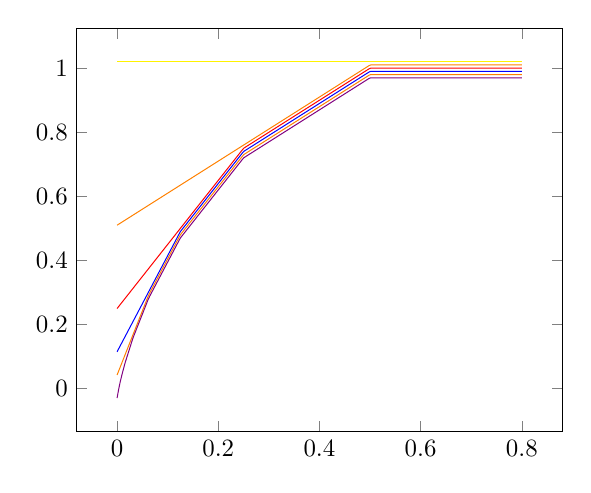
\begin{tikzpicture}[scale=0.9]
\begin{axis}[samples=250]
\addplot[yellow,domain=0:0.8] {1+0.02};

\addplot[orange,domain=0:0.8] {min(x+1/2, 1)+0.01};


\addplot[red,domain=0:0.8] {min(2*x+1/4, x+1/2, 1};
\addplot[blue,domain=0:0.8] {min(3*x+1/8,2*x+1/4, x+1/2, 1)-0.01};
\addplot[orange,domain=0:0.8] {min(4*x+1/16,3*x+1/8,2*x+1/4, x+1/2, 1)-0.02};

\addplot[violet,domain=0:0.8] {min(
10*x+1/1424,
9*x+1/712,
8*x+1/356,
7*x+1/128,
6*x+1/64,
5*x+1/32,
4*x+1/16,3*x+1/8,2*x+1/4, x+1/2, 1)-.03};


\end{axis}

\end{tikzpicture}
\caption{\small Tropical polynomials $\varphi_0,\dots,\varphi_4$ (top to bottom), and the limit tLs $\varphi$ (in violet). The points where the slope changes are  the tropical roots of $\varphi$, i.e.~the points $x=2^{-(i+1)}$, satisfying $ix+2^{-i}=(i+1)x+2^{-(i+1)}$.}
\label{fig:plot1}%\end{figure}%
\end{wrapfigure} %%

A \emph{tropical Laurent series} of one variable is a function $f:\Lawv\to\Lawv$ of shape $f(x)=\inf_{n\in\N}\{nx+\matr f_{n}\}$, with $\matr  f_{n}\in\Lawv$.
In other words, it is a ``limit'' of tropical polynomials of higher and higher degree.
E.g., the tLs $\varphi(x):=\inf_{n\in\N}\set{nx+2^{-n}}$ (see Fig.~\ref{fig:plot1}), that we will take as our running example, 
is the ``limit'' of the polynomials $\varphi_{n}$.
Since $\inf$s are not in general $\min$s, the behaviour of tLS may be less predictable than that of tropical polynomials~\cite{Porzio2021}. %For instance, tropical roots for tLs (see \cite{Porzio2021}) may also include limit points of their domain.

%
%
%We will take as our running example
%%given respectively by Equation~\ref{eq:polytrop} and Equation~\ref{eq:defTLS}.
%A positive $x\in[0,\infty)$ is said to be a (finite) \emph{tropical root} of a tropical Laurent series $f:\Lawv\to\Lawv$ iff $f$ is not differentiable at $x$ (w.r.t.\ the usual topology on $\BB R_{\geq0}$.This is equivalent to ask that the $\inf$ defining $f$ at $x$ is obtained \emph{at least} twice.{\color{red} \`e vero anche per TLS o solo per poly questo? Inoltre, Robol parla anche di finite end-points of the domain: nel nostro caso sarebbe $x=0$}

%\begin{example}\label{ex:famous_ex}
% The function $f:\Lawv\to\Lawv$ defined by $f(x):=\inf\limits_{n\in\N}\set{nx+\frac{1}{2^n}}$ is a tropical Laurent series.
%\end{example}

%By plotting its graph {\color{red}vogliamo plottarlo?}, we observe several properties that we will lift to the more general case that we will consider in the next lines, and this example will serve as running one.

%\begin{remark}%[Tropical Laurent series]
 Remark that the map $t^!:\Lawv^X\to\Lawv^Y$ introduced above from a matrix $t\in\HOM{\LREL_!}{X}{Y}$, corresponds to a tLs with \emph{possibly infinitely} many variables (in fact, as many as the elements of $X$). %In the following we will also refer to them as tLs. 
% We will call them simply \emph{tropical Laurent series (tLs)}.
% %Since in the general case of $\QREL$, $t^!$ is a Laurent series with operations in $Q$, let us call \emph{tropical Laurent series} the functions of shape $t^!$ for some $t\in\HOM{\LREL_!}{X}{Y}$.
%\end{remark}
%
%We find the usual notion of tLs of one variable as follows:
%\begin{remark}
By identifying $!\set{*}\simeq \N$ and $\Lawv^{\set{*}}\simeq\Lawv$, the tLs generated by the morphisms in $\HOM{\LREL_!}{\set{*}}{\set{*}}$ are exactly the %functions $f:\Lawv\to\Lawv$ of shape $f(x)=\inf_{n\in\N}\set{nx+\matr f(n)}$, for some $\matr f:\N\to\Lawv$, i.e.\ we recover the 
usual tLs's of one variable.
% \end{remark}
 \begin{remark}
 Our running example is indeed of shape $\varphi=t^!$, for $t\in\Lawv^{!\set{*}\times\set{*}}$, $t_{\mu,*}:=2^{-\# \mu}$.
 However, it is not the interpretation of a $\lam$-term, because its matrix $t$ is not discrete.
% Therefore $\LREL_!$ is not a full-complete model of $\STLC$.
\end{remark}



 In a similar way, tLs
$f:\Lawv^X\to\Lawv^Y$ 
 with \emph{finite} supports $\C F_b=\set{\mu\in!X\mid\matr f_{\mu,b}\neq\infty}$, and which have thus shape $f(x)_b=\min_{\mu\in\C F} \set{\mu x+ t_{\mu,b}}$, are generalisation of usual tropical polynomials to the case of possibly infinitely many variables.

% 
% , i.e.~for a \emph{finite} set $\C F\subseteq \, !X$.
%%Remark that we also find usual \emph{tropical polynomials} of tropical geometry as a particular case: they 
%correspond to the tLs for which the support $\set{n\in\N\mid\widehat f(n)\neq\infty}$ of $\widehat f$ is \emph{finite}. 
%Actually, for us \emph{tropical polynomial} will mean a function 
%\end{remark}

Looking at Fig~\ref{fig:plot1}, we see that $\varphi$, just like the polynomials $\varphi_{n}$, is non-decreasing and concave.
This is indeed always the case:

\begin{proposition}\label{prop:nondecr+conc}
 Any tLs $f:\Lawv^X\to\Lawv^Y$ is non-decreasing and concave, w.r.t.\ the pointwise order.
\end{proposition}

%In Example~\ref{ex:famous_ex}, 
Again by looking at Fig~\ref{fig:plot1} it appears that, \emph{far from $0$}, $\varphi$ behaves like some polynomials $\varphi_{n}$.
In particular, %for all $\epsilon >0$, $f$ coincides on $[\epsilon,\infty]$ with some polynomial $\varphi_{n}$. More, precisely, 
$\varphi$ coincides on $[\epsilon,\infty]$ with $\varphi_{n}$,
for $\epsilon \geq 2^{-(n+1)}$ (the smallest tropical root of $\varphi_{n}$).
However, at
%
%$x\in [\epsilon,\infty]$, with $\epsilon>0$
%It can be proven by hand that $\varphi(x)$ is a $\min$ for all $x>0$.
 $x=0$ we have that $\varphi(x=0)=\inf_{n\in\N} 2^{-n}=0$, and this is the only point where the $\inf$ is \emph{not} a $\min$.
Also, while the derivative of $f$ is bounded on all $(0,\infty)$, for $x\to 0^+$ it tends to $\infty$.
This phenomenon is reminiscent of \cite[Example 7]{Ehrhard2005},
%Differentials and Distances in Probabilistic Coherence Spaces. FSCD 2019
which actually motivated our first investigations.
In fact, this behaviour is shared by all tLs with \emph{finitely} many variables, as shown by the following result (we identify $!\set{1,\dots,k}\simeq \N^k$, so the matrix of a tLs $f$ with finitely many variables $x=x_1,\dots,x_k$ (and one output variable) is given as a $\matr f:\N^k\to\Lawv$, $f$ having shape $f(x)=\inf_{n\in \N^k}\set{nx+\matr f(n)}$, with $nx$ the scalar product).

\begin{theorem}\label{theorem:fepsilon}
 Let $k\in\N$ and $f:\Lawv^k\to\Lawv$ a tLs with matrix $\matr f:\N^k\to\Lawv$.
 For all $0<\epsilon<\infty$, there is a \emph{finite} $\C F_\epsilon \subseteq \N^k$ such that 
% 
% \begin{enumerate}
%  \item If $\C F_\epsilon=\emptyset$ then $f=\infty$ on all $\Lawv^k$;
%  \item If $f(x_0)=\infty$ for some $x_0\in[0,\infty)^k$, then $\C F_\epsilon=\emptyset$;
  %\item 
$f$ coincides on all $[\epsilon,\infty]^k$ with the tropical \emph{polynomial} $P_\epsilon(x):=\min_{n\in \C F_\epsilon}\set{nx+\matr f(n)}$.
% \end{enumerate}
\end{theorem}
\begin{proof}[Proof sketch]
Let $\C F_\epsilon$ be the set of $n\in\N^{k}$ such that 
$\widehat f(n)<\infty$ and $\widehat f(m)> \widehat f(n)+\epsilon$ holds for all $m\prec n$, where $\preceq$ is the pointwise order on $\N^k$.
The core of the proof is showing that this set is indeed finite and enough for computing $f$.
\end{proof}




\subsection{Continuity of tLs}\label{subsec:cont}%$\Lawv^{X}$ as a normed cone}

The tLs $\varphi$ is continuous on $\BB R_{\geq0}$ (w.r.t.\ the usual norm of real numbers).
By considering the usual norm $\norm{x}_\infty:=\sup_{a\in X} \absv{x_a}$ on $\Lawv^X$, we can generalise this property by dropping the case of $x$ having some $0$ coordinate:

\begin{theorem}\label{thm:cont}
 All tLs $f:\Lawv^X\to\Lawv$ are continuous on $\BB R_{>0}^X$, w.r.t.\ to the norm $\norm{\cdot}_\infty$.
\end{theorem}
\begin{proof}
 It follows after adapting [Proposition 4.4, \cite{Cobzas2017}] in order to prove that if a real-valued function on a locally convex topological $\BB R$-vector space is, locally around $x$, concave and bounded by a finite constant, then it is continuous at $x$.
\end{proof}

We conclude this subsection by noticing that $\Lawv^X$ with the usual $+$ and the usual $\cdot$ is a $\BB R_{\geq0}$-semimodule.
Together with the norm $\norm{\cdot}_\infty$, it can be proved that it is a Scott-complete \emph{normed cone} (see~\cite{Selinger2004}, or the appendix, for such notions).
Its cone structure induces an order on it, called its \emph{cone order}:
$x\leq y$ iff $y=x+z$ for some (unique) $z\in\Lawv^X$.
Such order actually coincides with the pointwise order on $\Lawv^X$.
This makes it a Scott-continuous dcpo.
Suitable categories of cones have been recently investigated as models of probabilistic computation (\cite{Crubillie2018, EhrPagTas2018, Ehrhard2020}).
Here we will just mention that:

\begin{theorem}\label{thm:ScottCont}
 All monotone (w.r.t.\ pointwise order) and $\norm{\cdot}_{\infty}$-continuous functions $f:(0,\infty)^X\to (0,\infty)$ are Scott-continuous.
 In particular, all tLs $f:\Lawv^X\to\Lawv$ are Scott-continuous on $(0,\infty)^X$ w.r.t.\ the pointwise orders.
\end{theorem}
\begin{proof}
 Use the fact, taken from \cite{Selinger2004}, that in a normed $\R_{\geq 0}$-cone $P$, considered with its cone-order, if every bounded directed net in $P$ admits a sup, and if $(v_i)_{i\in I}$ is a directed net in $P$ with an upper bound $v\in P$, then $\exists\bigvee_{i\in I} v_i \in P$ and, if $\inf_{i\in I} \norm{v-v_i} =0$, one has $\bigvee_{i\in I} v_i = v$.
\end{proof}



\subsection{Lipschitz-continuity of tLs}\label{sec:4C}%$\Lawv^{X}$ as a metric space.}


%The norm $\norm{\cdot}_\infty$ naturally induces a metric $\norm{x-y}_{\infty}$ over the spaces $\Lawv^{X}$.
We will show that tLs satisfy suitable Lipschitz properties w.r.t.\ $\norm{\cdot}_\infty$. 

Let us first look at tropical linear functions:


\begin{proposition}\label{prop:troplinear}
All tropical \emph{linear} functions $f: \Lawv^{X}\to \Lawv^{Y}$ are non-expansive.  
\end{proposition}
%\begin{proof}[Proof sketch]
%Using the fact that $f(\B x)_{b}= \inf_{a\in X}\matr f_{a,b}+\B x_{a}$,
%the problem reduces to checking that $|(\matr f_{a,b}-\B x_{a})- (\matr f_{a,b}-\B y_{a})| = |\B x_{a}-\B y_{a}|\leq \| \B x-\B y\|_{\infty}$.\end{proof}
This result shows that, in analogy with that happens in usual metric semantics, linear programs are interpreted by non-expansive functions. 
%\begin{proof}
%Using $f(\B x)_{b}= \inf_{a\in X}\matr f_{a,b}+\B x_{a}$,
%first observe that $|(\matr f_{a,b}-\B x_{a})- (\matr f_{a,b}-\B y_{a})| = |\B x_{a}-\B y_{a}|\leq \| \B x-\B y\|_{\infty}$; we now have
%$|f(\B x)_{b}-f(\B y)_{b}| \leq |(\inf_{a\in X}\matr f_{a,b}-\B x_{a})-(\inf_{a\in X}\matr f_{a,b}-\B y_{a})| \leq
%\sup_{a\in X}|(\matr f_{a,b}-\B x_{a})- (\matr f_{a,b}-\B y_{a})|\leq 
% \| \B x-\B y\|_{\infty}$.
%\end{proof}

%Before looking at what happens in the case of non-linear programs, let us make the metric structure of $\LREL$ explicit. 
The following proposition provides a useful characterization of the functional metrics in $\LREL$, relying on 
the bijection between $\HOM{\LREL}{X}{Y}$ and set of tropical linear functions from $\Lawv^{X}$ to $\Lawv^{Y}$.

\begin{proposition}
For all tropical linear functions $f,g:\Lawv^{X}\to \Lawv^{Y}$, $d_{\infty}(\matr f,\matr g)=d_\infty(f,g)$.% $\norm{ \matr f-\matr g}_{\infty} =  \sup_{x\in \Lawv^{X}} \norm{ f( x)-g(x)}_{\infty}$.
\end{proposition}

Let us now consider the case of bounded exponentials:
\begin{proposition}\label{prop:boundedlip}
If a tLs $f: \Lawv^{X}\to \Lawv^{Y}$ arises from a matrix $\matr f:!_{n}X\times Y\to \Lawv$, then $f$ is $n$-Lipschitz-continuous.
\end{proposition}
\begin{proof}[Proof sketch]
This follows from Proposition \ref{prop:troplinear} and the remark that, for all $x\in \Lawv^{X}$, $\norm{ !_{n} x-!_{n} y}_{\infty}\leq n\cdot \norm{ x- y}_{\infty}$, where $!_{n} x$ is the restriction of $! x$ to $\C M_{\leq n}(X)$.%
%Using the fact that $f(\B x)_{b}=\inf_{\mu\in \C M_{\leq n}(X)}\{ \matr f_{\mu,b}+ \mu (!_{n}\B x) \}$, where $!_{n}\B x\in \Lawv^{\C M_{\leq n}(X)}$ is given by 
%$(!_{n}\B x)_{[a_{1},\dots, a_{k}]}=\sum_{i=1}^{k}\B x_{a_{i}}$, 
%it suffices to check that $\| (!_{n}\B x)-(!_{n}\B y)\|_{\infty}\leq n\cdot \| \B x-\B y\|_{\infty}$ and apply Proposition \ref{prop:troplinear}.
\end{proof}
This result is perfectly analogous to what happens in the metric models discussed in Section \ref{section2}, the bounded exponentials $!_{n}$ playing the role of the re-scaling trick.

Observe that, for any tropical polynomial $\varphi:\Lawv^{X}\to \Lawv^{Y}$, the associated matrix has shape $!_{\mathrm{deg}(\varphi)}(X)\times Y\to \Lawv$ (as a monomial $\mu_ix+c_{i}$ yields a matrix entry on $!_{\#\mu_i}X\times Y$). Hence, using Proposition \ref{prop:boundedlip}, we have:
\begin{corollary}\label{prop:polylip}
For any tropical polynomial $\varphi:\Lawv^{X}\to\Lawv$, $\varphi$ is $\mathrm{deg}(\varphi)$-Lipschitz continuous.
\end{corollary}

Let us now look at what happens with tLs, i.e.~when considering the full exponential $!$.
As consequence of Theorem~\ref{theorem:fepsilon}, the tLs with \emph{finitely many} variables are always \emph{locally} Lipschitz on all $\BB R_{>0}$.
Actually, we can prove a more general statement, also covering the infinitary case.


\begin{theorem}\label{thmTLSlocLip}
 All tLs $\Lawv^X\to\Lawv$ are locally Lipschitz on $\BB R_{>0}^X$.
\end{theorem}
\begin{proof}[Proof sketch]
The core of the proof is a convex analysis argument (see the Appendix) showing that an arbitrary function $f:\Lawv^X\to\Lawv$ which is non-decreasing, concave and continuous, must be locally Lipschitz. 
\end{proof}


Finally, let us discuss the differential structure. The differential operator $D$ of $\LREL_{!}$ translates into a differential operator $D_{!}$ turing a tLs $f:\Lawv^{X}\to \Lawv^{Y}$ into a tLs $D_{!}f:\Lawv^{X}\times \Lawv^{X}\to \Lawv^{Y}$, linear in its first variable, and given by 
\begin{equation}
D_{!}f(x,y)_{b}=\inf_{a\in X, \mu\in !X}\left\{\matr f_{\mu+a}+x_{a}+\mu y\right\}
\end{equation}
One can check that, when $f$ is a tropical polynomial, $D_{!}f$ coincides with the standard tropical derivative (see e.g.~\cite{Grigoriev2017}).
Moreover, the Taylor formula \eqref{eq:taylorcat} yields a ``tropical'' Taylor formula for tLs of the form 
\begin{equation}
f(x)=\inf_{n}\left\{D_{!}^{(n)}(f)(!_{n}x,\infty)\right\}
\end{equation}
The following result shows that the distance between two tropical maps can be approximated using the terms appearing in their Taylor expansions:
\begin{proposition}
For all tLs $f,g: \Lawv^{X}\to \Lawv^{Y}$, and for all $n\in \BB N$, 
the functions $x\mapsto D_{!}^{(n)}(f)(!_{n}x,\infty)$ are $n$-Lipschitz. Moreover 
$\norm{ \matr f-\matr g}_{\infty}= \sup_{n} \norm{ {\delta^{(n)}f}- {\delta^{(n)}g}}_{\infty}$, 
where $\delta^{(n)}h$ indicates the matrix of $D_{!}^{(n)}h$.
%where $\delta^{(n)}f:( \Lawv^{X})^{n}\to \Lawv^{X}$ is the tropical linear function $\delta^{(n)}f(\B x_{1},\dots, \B x_{n})=
%(\Der^{(n)}f)(\B x_{1},\dots, \B x_{n}, \infty)$. 
\end{proposition} 


The results just presented translate into the following facts about the interpretation of higher-order programs:

\begin{corollary}
Let $\model A$ be a finite set.
\begin{enumerate}
\item $\model{\Gamma \vdash_{\BSTLC} M:A}^!:\Lawv^{\model\Gamma} \to \Lawv^{\model A}$ is a \emph{Lipschitz} map.
\item $\model{\Gamma \vdash_{\STLC} M:A}^!:\Lawv^{\model\Gamma} \to \Lawv^{\model A}$ is a \emph{locally} Lipschitz map.
\item $\Te{M}$ decomposes $\model{\Gamma \vdash_{\STLC} M:A}^!$ as an $\inf_{t\in\Te{M}}\model{\Gamma\vdash_{\STDLC} t:A}^!$ of \emph{tropical polynomials}, thus (as $\model A$ is finite), \emph{Lipschitz} functions.
\end{enumerate}
\end{corollary} 
\begin{proof}
1). As we observed, the interpretation $\model A$ of a bounded type is a finite set, hence $\model M$ must be a finite matrix  and  its corresponding linear map $\Lawv^{\model A} \to \Lawv^{\model B}$ is thus a tropical polynomial, so we apply Corollary~\ref{prop:polylip}.
2). It follows directly from Theorem~\ref{thmTLSlocLip}.
3). It follows from the easily checked fact that, for $(f_n)_{n\in\N}\subseteq\Lawv^{!X\times Y}$, we have $\left(\inf_{n\in\N} f_n\right)^!:\Lawv^X\to\Lawv^Y$, with $\left(\inf_{n\in\N} f_n\right)^!=\inf_{n\in\N} f_n^!$.
\end{proof}

Remark that the restriction to the ground type $*$ in (2) is without loss of generality, thanks Currying.

%Moreover, from Proposition \ref{prop:boundedlip}, we can also deduce the desired Lipschitz decomposition of the Taylor expansion (using Corollary~\ref{cor:T(M)=M}):

%\begin{corollary}\label{thm:M=infLip}
% If $\Gamma \vdash_{\STLC}M:A$, then $\model M^!: \model\Gamma \to \model A$ is an $\inf$ of \emph{Lipschitz} functions (via its Taylor expansion \eqref{eq:taylorcat}).
%\end{corollary}


%A consequence of this result is that the distance between two differential programs can always be approximated via bounded programs:
%\begin{corollary}
%For all $\lambda$-terms $M,N: A\to B$ of $\STDLC$, for all $\epsilon >0$, there exists $K\in \BB N$ such that 
%$|\|\model{M}-\model{N}\|_{\infty}- |\| \model{
%\end{corollary}
